\chapter{Laboratorio 1: Cammini disgiunti tramite algoritmo basato su pricing}


\begin{minted}[mathescape, fontsize=\small, xleftmargin=0.5em]{python}
import networkx as nx
import math
from networkx.algorithms.shortest_paths.weighted import dijkstra_path
\end{minted}


Definiamo una funzione per generare grafi in una  forma precisa, ossia a 
\textit{doppio ventaglio}: 

\begin{minted}[mathescape, fontsize=\small, xleftmargin=0.5em]{python}
def doubleFan(k):
    G = nx.DiGraph()
    G.add_nodes_from(['s', 't', 'x', 'y'])
    G.add_nodes_from(['a' + str(i) for i in range(k)])
    G.add_nodes_from(['b' + str(i) for i in range(k)])
    G.add_edges_from([('s', 'a' + str(i)) for i in range(k)])
    G.add_edges_from([('a' + str(i), 'x') for i in range(k)])
    G.add_edges_from([('y', 'b' + str(i)) for i in range(k)])
    G.add_edges_from([('b' + str(i), 't') for i in range(k)])
    G.add_edge('x', 'y')
    return G
\end{minted}

\begin{minted}[mathescape, fontsize=\small, xleftmargin=0.5em]{python}
nx.draw(doubleFan(2))
\end{minted}
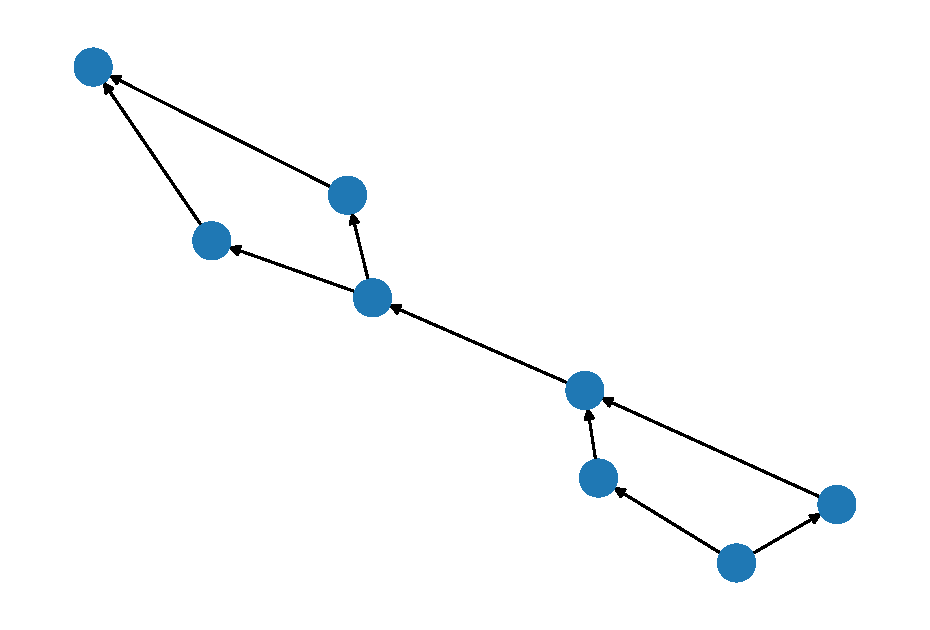
\includegraphics[width=0.3 \linewidth]{labs/figures/lab1_figure3_1.pdf}


\begin{minted}[mathescape, fontsize=\small, xleftmargin=0.5em]{python}
nx.draw(doubleFan(4))
\end{minted}
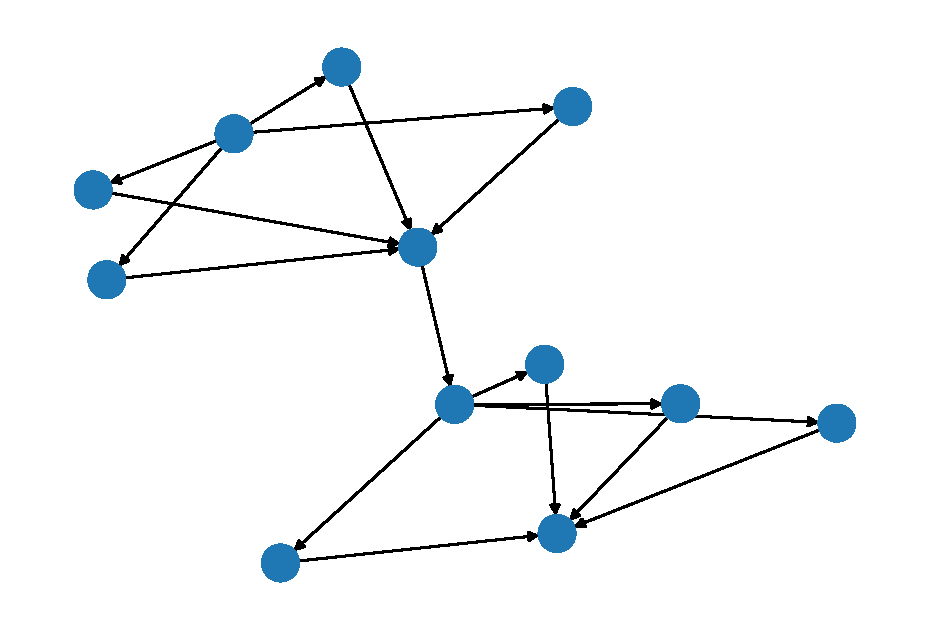
\includegraphics[width=0.3 \linewidth]{labs/figures/lab1_figure4_1.pdf}



\begin{minted}[mathescape, fontsize=\small, xleftmargin=0.5em]{python}
nx.draw(doubleFan(8))
\end{minted}
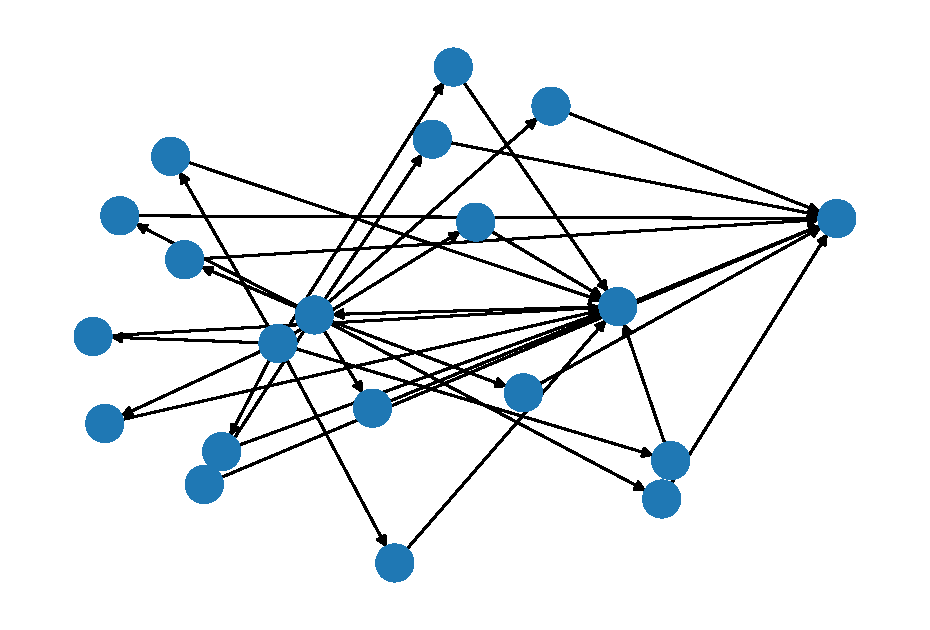
\includegraphics[width=0.3 \linewidth]{labs/figures/lab1_figure5_1.pdf}


Definiamo, quindi, una funzione che implementa \textsc{PricedDisjointPaths}: 


\begin{minted}[mathescape, fontsize=\small, xleftmargin=0.5em]{python}
def greedyDisjointPaths(G_original, sourceTargetPairs, c = 1):
    G = G_original.copy()
    result = []
    beta = math.pow(G.number_of_edges(), 1 / (c + 1))
    # Set all lengths to 1 and all congestion to 0
    for u,v,d in G.edges(data = True):
        d['length'] = 1
        d['congestion'] = 0
    # Main cycle
    while True:
        minPath = None
        for pairIndex in range(len(sourceTargetPairs)):
            try:
                source = sourceTargetPairs[pairIndex][0]
                target = sourceTargetPairs[pairIndex][1]
                path = dijkstra_path(G, source, target, 'length')
            except:
                pass
            else:
                pathLength = 0
                for i in range(len(path) - 1):
                    pathLength += G[path[i]][path[i+1]]['length']
                if minPath == None or pathLength < minPathLength:
                    minPath = path
                    minPathLength = pathLength
                    minPathIndex = pairIndex
        if minPath == None:
            break
        result.append(minPath)
        sourceTargetPairs.pop(minPathIndex)
        for i in range(len(path) - 1):
            x1 = path[i]
            x2 = path[i+1]
            G[x1][x2]['length'] *= beta
            G[x1][x2]['congestion'] += 1
            if G[x1][x2]['congestion'] == c:
                G.remove_edge(x1, x2)
    return result
\end{minted}



\begin{minted}[mathescape, fontsize=\small, xleftmargin=0.5em]{python}
g = doubleFan(2)
nx.draw(g, with_labels = True)
\end{minted}
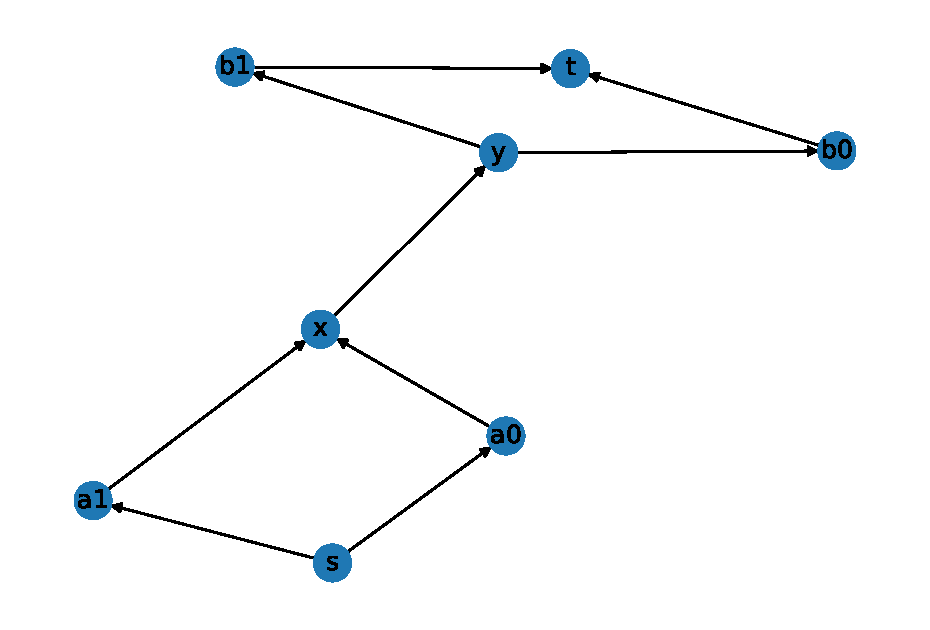
\includegraphics[width=0.5 \linewidth]{labs/figures/lab1_figure7_1.pdf}



\begin{minted}[mathescape, fontsize=\small, xleftmargin=0.5em]{python}
greedyDisjointPaths(g, [('s', 't')]*11, c = 10)
\end{minted}
\begin{minted}[fontsize=\small, xleftmargin=0.5em, mathescape, frame = leftline]{text}
[['s', 'a0', 'x', 'y', 'b0', 't'],
 ['s', 'a1', 'x', 'y', 'b1', 't'],
 ['s', 'a0', 'x', 'y', 'b0', 't'],
 ['s', 'a1', 'x', 'y', 'b1', 't'],
 ['s', 'a0', 'x', 'y', 'b0', 't'],
 ['s', 'a1', 'x', 'y', 'b1', 't'],
 ['s', 'a0', 'x', 'y', 'b0', 't'],
 ['s', 'a1', 'x', 'y', 'b1', 't'],
 ['s', 'a0', 'x', 'y', 'b0', 't'],
 ['s', 'a1', 'x', 'y', 'b1', 't']]
\end{minted}



\begin{minted}[mathescape, fontsize=\small, xleftmargin=0.5em]{python}
g = doubleFan(4)
nx.draw(g, with_labels = True)
\end{minted}
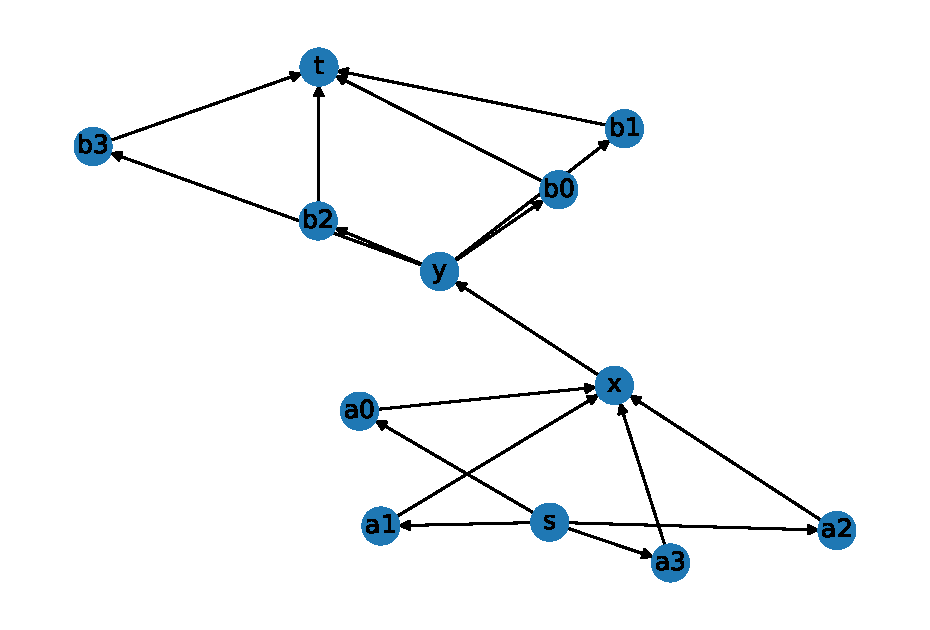
\includegraphics[width=0.5 \linewidth]{labs/figures/lab1_figure9_1.pdf}



\begin{minted}[mathescape, fontsize=\small, xleftmargin=0.5em]{python}
greedyDisjointPaths(g, [('s', 't')]*11, c = 10)
\end{minted}
\begin{minted}[fontsize=\small, xleftmargin=0.5em, mathescape, frame = leftline]{text}
[['s', 'a0', 'x', 'y', 'b0', 't'],
 ['s', 'a1', 'x', 'y', 'b1', 't'],
 ['s', 'a2', 'x', 'y', 'b2', 't'],
 ['s', 'a3', 'x', 'y', 'b3', 't'],
 ['s', 'a0', 'x', 'y', 'b0', 't'],
 ['s', 'a1', 'x', 'y', 'b1', 't'],
 ['s', 'a2', 'x', 'y', 'b2', 't'],
 ['s', 'a3', 'x', 'y', 'b3', 't'],
 ['s', 'a0', 'x', 'y', 'b0', 't'],
 ['s', 'a1', 'x', 'y', 'b1', 't']]
\end{minted}

